\documentclass[12pt,letterpaper]{article}

\newcommand{\IncludePath}{../include}
\usepackage{extsizes}
\usepackage{titling}

\usepackage{amssymb,amsmath,amsthm}
\usepackage{enumerate}
\usepackage[margin=1in]{geometry}
\usepackage{graphicx,ctable,booktabs}
\usepackage{fancyhdr}
\usepackage[utf8]{inputenc}

\makeatletter
\newenvironment{problem}{\@startsection
       {section}
       {1}
       {-.2em}
       {-3.5ex plus -1ex minus -.2ex}
       {2.3ex plus .2ex}
       {\pagebreak[3]
       \large\bf\noindent{Problem }
       }
       }
\makeatother

\pagestyle{fancy}
\lhead{\thetitle}
\chead{}
\rhead{\thepage}
\lfoot{\small\scshape Grade 4 Olympic Math}
\cfoot{}
\rfoot{}
\renewcommand{\headrulewidth}{.3pt}
\renewcommand{\footrulewidth}{.3pt}
\setlength\voffset{-0.25in}
\setlength\textheight{648pt}
\setlength\headheight{15pt}


\title{Quiz 1: Geometry}
\author{Name: \underline{\hspace{5cm}} \OutOf{10}}
\date{November 26, 2016}

\begin{document}

\newcommand*\circleletter[1]{%
  \begin{tikzpicture}[baseline=(C.base)]
    \node[draw,circle,inner sep=1pt](C) {#1};
  \end{tikzpicture}}

\maketitle

\thispagestyle{empty}

\section*{Instructions}
\begin{itemize}
  \item The quiz is marked out of 10.
  \item Problem 2 is a bonus question. The maximum achievable score is 12.
  \item (Optional) Show work on the scrap paper. Part marks are awarded for
  work done.
  \item All angles that look right are right. All lines that look parallel are
  parallel.
  \item Calculators are not permitted. Reference formulas on bottom of back
  page.
\end{itemize}

\begin{problem}{Toronto\hfill/4}
\begin{figure}[h]
  \begin{center}
    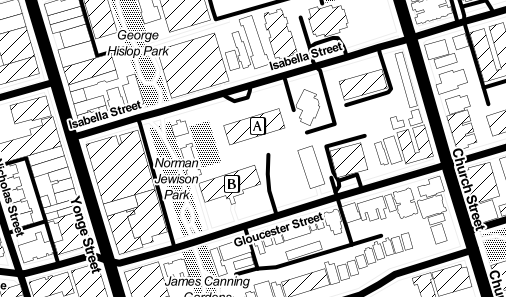
\includegraphics[trim=50 50 50 50, clip, width=.5\textwidth]{toronto.png}
  \end{center}
  \caption{Map from OpenStreetMap}
\end{figure}

 Look at the map of this block in Toronto. Circle the correct response.

 \begin{enumerate}
  \item At what kind of angle do Isabella Street and Yonge Street intersect?

  \hfill Acute~~Right~~Obtuse~~Straight~~Reflex

  \item What kind of shape is Building~\circleletter{A}?
  \hfill Rhombus~~Kite~~Rectangle

  \item What is the sum of interior angles for Building~\circleletter{A}? \hfill
  \SI{90}{\degree}~~\SI{180}{\degree}~~\SI{360}{\degree}~~\SI{540}{\degree}

  \item Which building has greater area?
  \hfill Building~\circleletter{A}~~Building~\circleletter{B}
 \end{enumerate}
\end{problem}

\begin{problem}{Triangle\hfill/2}
 A right triangle has base length \SI{10}{\meter} and height \SI{10}{\meter}.

 \begin{enumerate}
  \item What is its area?
  \hfill \underline{\hspace{3em}} \si{\meter^2}
  \item How many interior acute angles does the triangle have?
  \hfill \underline{\hspace{3em}}
 \end{enumerate}
\end{problem}

\begin{problem}{Garden\hfill/5}
  \begin{center}
    \begin{tikzpicture}
      \coordinate (B) at (3,0);
      \coordinate (A) at (2,0);
      \coordinate (C) at (1,2);
      \draw[step=1cm,gray] (-0.3,-0.3) grid (5.3,4.3);
      \draw[line width=1mm] (0,0) -- (0,4) -- (5,4) -- (5,0) -- (4,2) -- (3,0)
      -- (2,0) -- (1,2) -- cycle;
      \pic [draw, "\(\alpha\)", line width=0.4mm, angle radius=0.6cm]
      {angle = B--A--C};
    \end{tikzpicture}
  \end{center}

 Look at the map of Vegeta's vegetable garden. The part enclosed in the bold
 lines is the garden itself. Each grid square represents \SI{1}{\meter^2}. One
 angle is marked.

 \begin{enumerate}
  \item What kind of angle is the marked angle \(\alpha\)? (circle one)

  \hfill Acute~~Right~~Obtuse~~Straight~~Reflex

  \item The angle supplementary to \(\alpha\) is \SI{63}{\degree}. What is the
  measure of \(\alpha\)?
  \hfill \blankC \si{\degree}

  \item How many sides does this garden have? \hfill \blankC

  \item How many of the garden's interior angles are reflex angles?
  \hfill \blankC

  \item What is the area of this garden? \hfill \blankC \si{\meter^2}
\end{enumerate}

\end{problem}

\begin{problem}{Challenge\hfill/1}
 Two angles are complementary. One is \SI{18}{\degree} greater than the other.
 What are the two angles? \vspace{1ex}

 \hfill \blankC \si{\degree}, \blankC \si{\degree}
\end{problem}

\vspace{1em}\noindent\underline{Reference}

\noindent Area formulas: \(A_\Delta=\frac{1}{2}bh\), \(A_\square=\ell w\),
\(A_\text{parallelogram}=bh\),
\(A_\text{trapezoid}=\frac{1}{2}\left(b_1+b_2\right)h\)

\noindent Interior angle sum: \(\mathrm{AS}=\SI{180}{\degree} (n-2)\)

\noindent Complementary angles sum to \(\SI{90}{\degree}\)

\noindent Supplementary angles sum to \(\SI{180}{\degree}\)

\end{document}
